\documentclass[titlepage = firstcover]{scrartcl}
\usepackage[aux]{rerunfilecheck}
\usepackage{fontspec}
\usepackage[main=ngerman, english, french]{babel}

% mehr Pakete hier
\usepackage{expl3}
\usepackage{xparse}

%Mathematik------------------------------------------------------
\usepackage{amsmath}   % unverzichtbare Mathe-Befehle
\usepackage{amssymb}   % viele Mathe-Symbole
\usepackage{mathtools} % Erweiterungen für amsmath
\usepackage{dsfont}
\usepackage[
  math-style=ISO,    % \
  bold-style=ISO,    % |
  sans-style=italic, % | ISO-Standard folgen
  nabla=upright,     % |
  partial=upright,   % /
]{unicode-math}% "Does exactly what it says on the tin."
\usepackage[section, below]{placeins}

% Laden von OTF-Mathefonts
% Ermöglich Unicode Eingabe von Zeichen: α statt \alpha

\setmathfont{Latin Modern Math}
%\setmathfont{Tex Gyre Pagella Math} % alternativ zu Latin Modern Math
\setmathfont{XITS Math}[range={scr, bfscr}]
\setmathfont{XITS Math}[range={cal, bfcal}, StylisticSet=1]

\AtBeginDocument{ % wird bei \begin{document}
  % werden sonst wieder von unicode-math überschrieben
  \RenewDocumentCommand \Re {} {\operatorname{Re}}
  \RenewDocumentCommand \Im {} {\operatorname{Im}}
}
\usepackage{mleftright}
\setlength{\delimitershortfall}{-1sp}
\usepackage[version=4]{mhchem}

%Sprache----------------------------------------------------------
\usepackage{microtype}
\usepackage{xfrac}
\usepackage[autostyle]{csquotes}    % babel
\usepackage[german, unicode, pdfusetitle]{hyperref}
\usepackage{bookmark}
\usepackage[shortcuts]{extdash}
%Einstellungen hier, z.B. Fonts
\usepackage{booktabs} % Tabellen

\setlength{\parindent}{0pt}

\title{US2 - Scanverfahren in der Ultraschalltechnik}
\author{
  David Gutnikov\\
  \href{mailto:david.gutnikov@udo.edu}{david.gutnikov@udo.edu}\\
  Lasse Sternemann\\
  \href{mailto:lasse.sternemann@udo.edu}{lasse.sternemann@udo.edu}
}
\date{Bearbeitet am 7.07.2020}

\begin{document}
    \maketitle
    \newpage
    \tableofcontents
    \newpage

    \section{Auswertung}
        Aufgrund mangelnder Kompetenz ist dem Programm nicht die Laufzeit des Schalls, sondern direkt die Tiefe der Löcher entnommen worden. Deswegen werden diese Werte direkt mit den mit Hilfe
        einer Schiebelehre gemessenen Werten verglichen und anschließend die theoretische Laufzeit des Schalls bei entsprechender Tiefe berechnet.

        \FloatBarrier

        \begin{figure}[h]
          \centering
          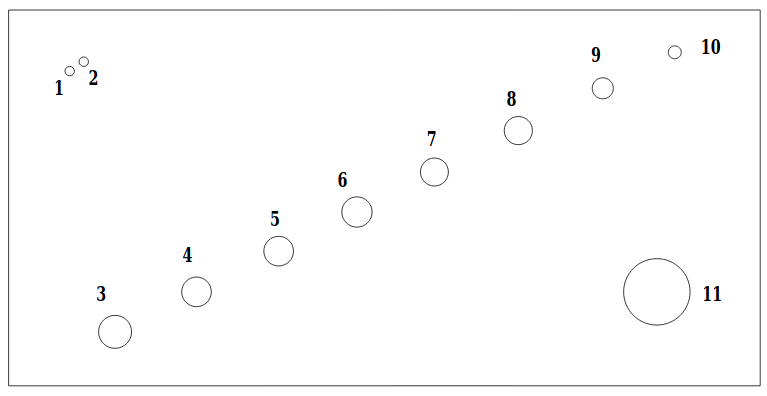
\includegraphics[width = 0.8\textwidth]{Bilder/DerBlock.png}
          \caption{In der Abbildung ist der untersuchte Acrylblock zu sehen.}
          \label{fig:DerBlock}
        \end{figure}

        \FloatBarrier

        \noindent


        \subsection{Amplituden-Scan}
            In der ersten Tabelle \ref{tab:Abstand1} sind die Abstände der Löcher 3, 4, 5, 6 und 7 von der in Skizze \ref{fig:DerBlock} unten liegenden Seite per Messung mit der Schiebelehre und per Messung durch den 
            Ampliuden-Scan eingetragen. Zusätzlich wird die Abweichung des per Amplituden-Scans gemessenen Abstands zum Wert der Schiebelehre, sowie die theoretische Laufzeit der Schallwelle im
            Acrylblock berechnet und in die Tabelle eingetragen. Zur Berechnung der Laufzeit wird Formel x nach t umgestellt.

            \begin{table}[h]
                \centering
                \caption{In der Tabelle sind die gemessenen Abstände, sowie deren Abweichung und die theoretische Laufzeit des Schalls, unter Vorraussetzung der richtig gewählten spezifischen Schallgeschwindigkeit im Programm, eingetragen.}
                \label{tab:Abstand1}

                \begin{tabular}{c c c c c}
                    \toprule
                    {Loch} & {Abstand SL [mm]} & {Abstand A-Scan [mm]} & {Abweichung [\%]} & {Laufzeit [$\mu$s]}  \\
                    \midrule
                    3   &   13,30$\pm$0,02   &   16$\pm$1  &   20,30   &   11.99$\pm$0,75   \\
                    4   &   21,80$\pm$0,02   &   24$\pm$1  &   10,09   &   17,98$\pm$0,75   \\
                    5   &   30,14$\pm$0,02   &   33$\pm$1  &   9,49    &   24,72$\pm$0,75   \\
                    6   &   38,60$\pm$0,02   &   41$\pm$1  &   6,22    &   30,71$\pm$0,75   \\
                    7   &   46,58$\pm$0,02   &   49$\pm$1  &   5,20    &   36,70$\pm$0,75   \\       
                    \bottomrule
                \end{tabular}

            \end{table}

            \FloatBarrier
            \noindent




        \end{document}
            